\documentclass[tikz,border=10pt]{standalone}
\usetikzlibrary{calc}
\begin{document}
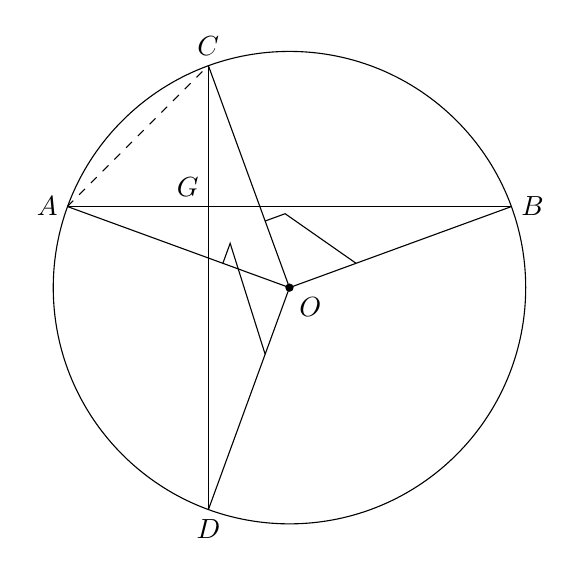
\begin{tikzpicture}[scale=1]
  \coordinate (O) at (0,0);
  \coordinate (A) at (-2.82,1.03);
  \coordinate (B) at (2.82,1.03);
  \coordinate (C) at (-1.03,2.82);
  \coordinate (D) at (-1.03,-2.82);
  \coordinate (G) at (-1.03,1.03);

  \draw (O) circle (3);

  \draw[dashed] (A) -- (C);
  \draw (O) -- (A);
  \draw (O) -- (B);
  \draw (O) -- (C);
  \draw (O) -- (D);
  \draw (A) -- (B);
  \draw (C) -- (D);

  % right angle between OC and OB
  \draw ($(O)!0.3!(C)$) -- ($($(O)!0.3!(C)$)!0.3!90:(O)$) -- ($(O)!0.3!(B)$);
  % right angle between OA and OD
  \draw ($(O)!0.3!(A)$) -- ($($(O)!0.3!(A)$)!0.3!90:(O)$) -- ($(O)!0.3!(D)$);

  \fill (O) circle (1.5pt);

  \node[above] at (C) {$C$};
  \node[left] at (A) {$A$};
  \node[right] at (B) {$B$};
  \node[below] at (D) {$D$};
  \node[below right] at (O) {$O$};
  \node[above left] at (G) {$G$};
\end{tikzpicture}
\end{document}
